\documentclass[tikz,border=7pt]{standalone}

\usepackage{iftex}
\ifPDFTeX
  \PackageError{matrix-figure}{This figure requires XeTeX or Tectonic}{Compile with xelatex or tectonic.}
\fi
\usepackage{fontspec}
\usepackage{xeCJK}
\usepackage{amsmath}
\usepackage{unicode-math}
\usepackage{xcolor}
\usepackage{tikz}
\usetikzlibrary{arrows.meta,positioning}

\providecommand{\FigureUseLocalFonts}{0}
\ifnum\FigureUseLocalFonts=1
  \setmainfont{NotoSansCJKtc-Regular.otf}[Path=\FigureSansFontPath]
  \setsansfont{NotoSansCJKtc-Regular.otf}[Path=\FigureSansFontPath,BoldFont=NotoSansCJKtc-Bold.otf]
  \setCJKmainfont{NotoSansCJKtc-Regular.otf}[Path=\FigureSansFontPath]
  \setCJKsansfont{NotoSansCJKtc-Regular.otf}[Path=\FigureSansFontPath,BoldFont=NotoSansCJKtc-Bold.otf]
  \setmathfont{STIXTwoMath.otf}[Path=\FigureMathFontPath]
\else
  \setmainfont{Noto Sans CJK TC}
  \setsansfont{Noto Sans CJK TC}
  \setCJKmainfont{Noto Sans CJK TC}
  \setCJKsansfont{Noto Sans CJK TC}
  \setmathfont{STIX Two Math}
\fi

\definecolor{FigureInk}{HTML}{253142}
\definecolor{RowShade}{gray}{0.84}
\definecolor{ColumnShade}{gray}{0.72}
\definecolor{ResultShade}{gray}{0.56}
\definecolor{PanelFill}{gray}{0.96}

\newcommand{\MatrixCell}[2]{%
  \tikz[baseline=(value.base)]{\node[fill=#1,rounded corners=0.4pt,inner sep=2.2pt,
    minimum width=1.35em,minimum height=1.35em] (value) {$#2$};}%
}
\newcommand{\RowCell}[1]{\MatrixCell{RowShade}{#1}}
\newcommand{\ColumnCell}[1]{\MatrixCell{ColumnShade}{#1}}
\newcommand{\ResultCell}[1]{\MatrixCell{ResultShade}{#1}}

\begin{document}
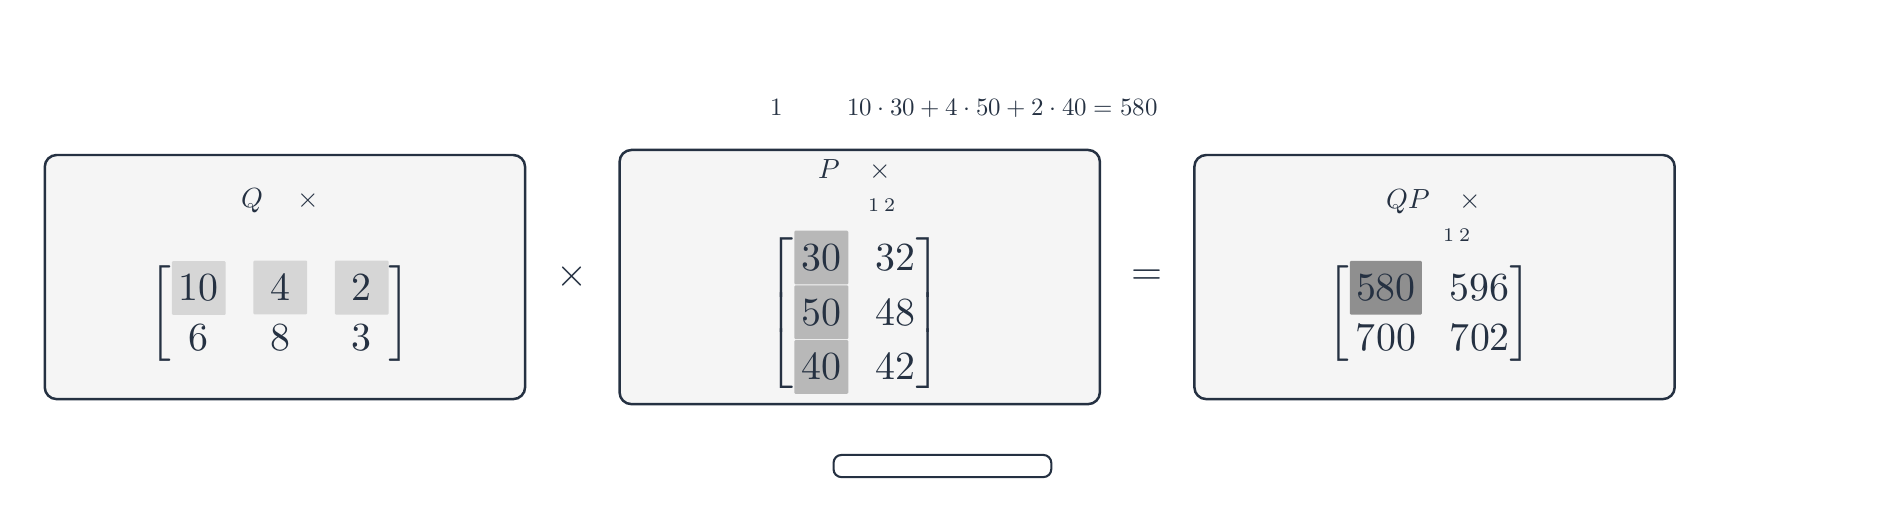
\begin{tikzpicture}[
  font=\sffamily,
  text=FigureInk,
  panel/.style={draw=FigureInk,line width=0.9pt,rounded corners=1.5mm,fill=PanelFill,
                minimum height=3.1cm,align=center},
]
  \node[font=\bfseries\Large,align=center,text width=23cm] at (11.5,6.0)
    {商品索引逐項配對並加總，輸出保留門市與月份索引};
  \node[font=\small,align=center] at (11.5,5.10)
    {甲門市在第 $1$ 個月份的總成本：$10\cdot30+4\cdot50+2\cdot40=580$};

  \node[panel,minimum width=6.1cm] (Q) at (3.15,2.95) {%
    \begin{minipage}{5.5cm}\centering
      \textbf{數量 $Q$：門市 $\times$ 商品}\\[4pt]
      \scriptsize 欄依序為紙、筆、冊；列依序為甲門市、乙門市\\[6pt]
      \Large$\begin{bmatrix}
        \RowCell{10}&\RowCell{4}&\RowCell{2}\\
        6&8&3
      \end{bmatrix}$
    \end{minipage}
  };
  \node[font=\Large] at (6.80,2.95) {$\times$};
  \node[panel,minimum width=6.1cm] (P) at (10.45,2.95) {%
    \begin{minipage}{5.5cm}\centering
      \textbf{單價 $P$：商品 $\times$ 月份}\\[4pt]
      \scriptsize 列：紙、筆、冊；欄：第 $1$、$2$ 月\\[6pt]
      \Large$\begin{bmatrix}
        \ColumnCell{30}&32\\
        \ColumnCell{50}&48\\
        \ColumnCell{40}&42
      \end{bmatrix}$
    \end{minipage}
  };
  \node[font=\Large] at (14.10,2.95) {$=$};
  \node[panel,minimum width=6.1cm] (QP) at (17.75,2.95) {%
    \begin{minipage}{5.5cm}\centering
      \textbf{總成本 $QP$：門市 $\times$ 月份}\\[4pt]
      \scriptsize 列：甲、乙門市；欄：第 $1$、$2$ 月\\[6pt]
      \Large$\begin{bmatrix}
        \ResultCell{580}&596\\
        700&702
      \end{bmatrix}$
    \end{minipage}
  };

  \node[draw=FigureInk,line width=0.75pt,rounded corners=1mm,fill=white,
        font=\scriptsize,inner xsep=7pt,inner ysep=4pt] at (11.5,0.55)
    {淺灰列與中灰行都按「紙、筆、冊」排序；深灰輸出格是三項費用的總和。};
\end{tikzpicture}
\end{document}
